\subsection{Hipótese 2}
\label{sec:resultados-hipotese-2}

Nossa hipótese 2 afirma que a aprendizagem dos alunos de DS (não de DA) é maior nas aulas que abordam algoritmos explicitamente (\eg, ``MeanShift e DBSCAN'') do que naquelas com tópicos mais abstratos (\eg, ``o funcionamento de um neurônio'').

A verificação dessa hipótese é similar à primeira, exceto que dessa vez segmentamos os dados em aulas que envolvem explicitamente algoritmos ou não:
\begin{align*}
	H_0&: \mu_a = \mu_{\neg a} \\
	H_a&: \mu_a > \mu_{\neg a},
\end{align*}
onde $\mu_a$ é a média da população de aulas contendo a componente ``algoritmo'' e $\mu_{\neg a}$, a média populacional das demais aulas.

Na Seção~\ref{sec:resultados} nós mostramos como essas aulas foram identificadas (coluna \foreign{algorithm} do conjunto de dados), restando agora executar a segmentação e o teste t.

\begin{figure}
	\centering
	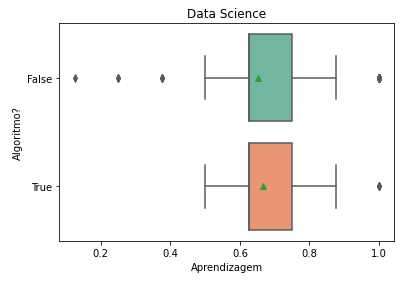
\includegraphics[width=0.45\textwidth]{ds-boxplot-by-algorithm}
	\caption{Distribuição da aprendizagem nos cursos de DS para as aulas de algoritmos (\foreign{true} no eixo vertical) e as demais.}
	\label{fig:dist-hipotese-2}
\end{figure}

A Figura~\ref{fig:dist-hipotese-2} e a Tabela~\ref{tab:dist-hipotese-2} apresentam a distribuição da aprendizagem das aulas de algoritmos e das demais do curso de DS.

\begin{table}
	\centering
	\begin{minipage}[t]{0.46\textwidth}
		\caption{Tamanho da amostra (\#), média e desvio-padrão da aprendizagem em DS.}
		\label{tab:dist-hipotese-2}
		\begin{tabular}{lrrr}
			\toprule
			Algoritmo? & \# & $\bar{a}$ & $s_a$ \\
			\midrule
			Sim &  110 &  $1,3\pm 0,2$ & 0,88 \\
			Não & 1653 & $1,25\pm 0,04$ & 0,88 \\
			\bottomrule
		\end{tabular}
	\end{minipage}\hfill
	\begin{minipage}[t]{0.46\textwidth}
		\caption{Estatísticas de teste da hipótese 2.}
		\begin{tabular}{lcc}
		\toprule
		Curso & Valor $p$   & Estatística $t$ \\
		\midrule
		DS    & $0,41$      & $0,83$ \\ 
		\bottomrule
		\end{tabular}
	\end{minipage}
\end{table}

O curso de DA não tem ênfase em algoritmos.
Por isso não propusemos fazer teste análogo nele.
De fato, podemos verificar no conjunto de dados que a quantidade de aulas com o atributo \foreign{algorithm} = \foreign{true} é zero.

Note, na Tabela~\ref{tab:dist-hipotese-2}, que a média amostral das aulas de algoritmo reside no intervalo $1,1 \le \mu_a \le 1,5$, que contém a média amostral das demais aulas.
Além disso, os desvios-padrão são similares.
Isso evidencia que as duas amostras têm origem na mesma população.
Porém, apenas o teste t nos permitirá afirmar.

Ao efetuarmos o teste de hipótese, obtivemos valor-$p$ de 41\%.
Ou seja, a probabilidade de observarmos a média $\bar a = 1,3 \pm 0,2$ numa amostra de uma população com média $\mu_a = 1,25 \pm 0,04$ é de 41\%, acima do nível de significância de 5\% assumido.
Logo, podemos afirmar que as duas amostras advém da mesma população (mais rigorosamente, nossos dados não fornecem evidência suficiente para rejeitar $H_0$).
Consequentemente, \emph{não} há diferença de aprendizagem entre as aulas de algoritmos e as demais.

Utilizando novamente a teoria do valor da expectativa para interpretar esse resultado, isso significa que a instrumentalidade das componentes relacionadas a algoritmos é equivalente àquela associada às demais aulas.
Ou seja, o aluno não vê distinção entre essas aulas e, com isso, apresenta o mesmo nível de motivação para aprender.